\documentclass[spanish,notes=hide]{beamer}

%Para crear una versión 'handout' (Copyright: Diego Berrueta)
%\documentclass[handout,notes=show]{beamer}

\usetheme{Marburg}

\usepackage[spanish]{babel}
\usepackage[utf8]{inputenc}
\usepackage{listings}
\usepackage{graphicx}
\usepackage{colortbl}
\usepackage{array}
\usepackage{eurosym}

\title{SWAML}
\subtitle{Semantic Web Archive of Mailing Lists}
\author{Sergio Fern\'andez}
\institute{%
        \email{sergio.fernandez@fundacionctic.org}\\
	Departamento I+D+i (Fundación CTIC)\\
	\vspace{1cm}
	E.U.I.T.I.O (Universidad de Oviedo)\\
	\vspace{1cm}
	\href{http://swaml.berlios.de/}{\begin{Large}\textbf{http://swaml.berlios.de/}\end{Large}}\\
        \vspace{0.5cm}
}
\date{11 de Mayo de 2007}

\begin{document}


%tableofcontents

%\AtBeginSection[]
%{
%   \begin{frame}
%       \frametitle{Tabla de contenidos}
%       \tableofcontents[currentsection]
%   \end{frame}
%}

%\AtBeginSubsection[] 
%{
%   \begin{frame}
%       \frametitle{Tabla de contenidos}
%       \tableofcontents[currentsection,currentsubsection]
%   \end{frame}
%}

%listings

\definecolor{darkred}{rgb}{0.5, 0, 0}
\definecolor{violet}{rgb}{1, 0, 1}
\definecolor{green}{rgb}{0.3, 0.95, 0.3}
\definecolor{listinggray}{gray}{0.97}

\lstset{
	basewidth=0.50em,
	backgroundcolor=\color{listinggray},
	basicstyle=\footnotesize\ttfamily,
	keywordstyle=\bfseries,
	stringstyle=\itshape,
	commentstyle=\itshape,
	showspaces=false,
	showtabs=false,
	showstringspaces=false,
	frame=trbl,
	extendedchars=true,
	numbers=none,
	aboveskip=0.5cm,
	belowskip=0.5cm,
	xleftmargin=0cm,
	xrightmargin=0cm
}

\lstdefinelanguage{mbox}{%no funciona!
	morekeywords = {From, Message, Date, Organization, To, Subject }
}

\lstdefinelanguage{SPARQL}{%
	morekeywords = {PREFIX, SELECT, DISTINCT, WHERE }
}


\maketitle

\section{Introducción}
\frame
{
  \frametitle{Introducción}

  \begin{itemize}
   \item<2-> \begin{large}\textbf{Situación actual:}\end{large}
	\begin{itemize}
	  \item \begin{large}miles de listas de correo\end{large}
	  \item \begin{large}publicación (sintáctica) en (X)HTML\end{large}
	\end{itemize}
   \vspace{1cm}
   \item<3-> \textbf{Problemas:}
	\begin{itemize}
	  \item \begin{large}pérdida de información\end{large}
	  \item \begin{large}marcado sin ningún valor semántico\end{large}
	  \item \begin{large}problemas usando motores de búsqueda convencionales\end{large}
	\end{itemize}
  \end{itemize}
}
\frame
{
  \frametitle{Archivos de una lista de correo en HTML}

  \begin{center}
    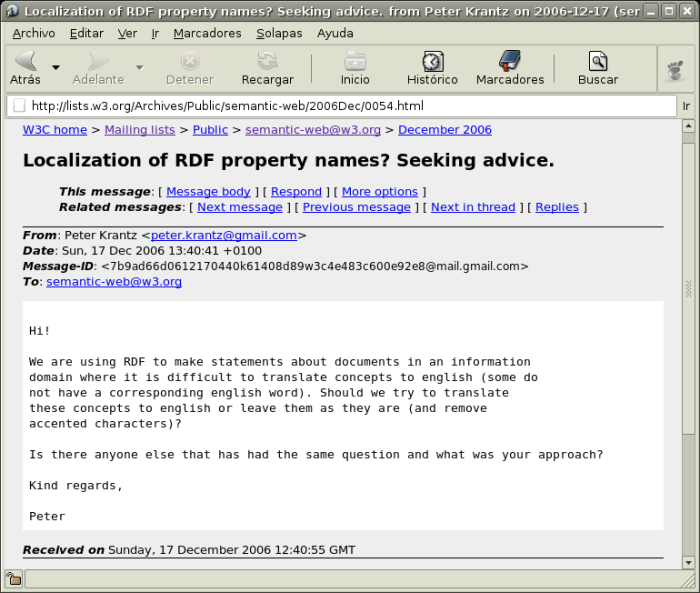
\includegraphics[width=0.8\textwidth]{images/lista-html.png}
  \end{center}
}
\frame
{
  \frametitle{Búsquedas caóticas}

  \begin{center}
    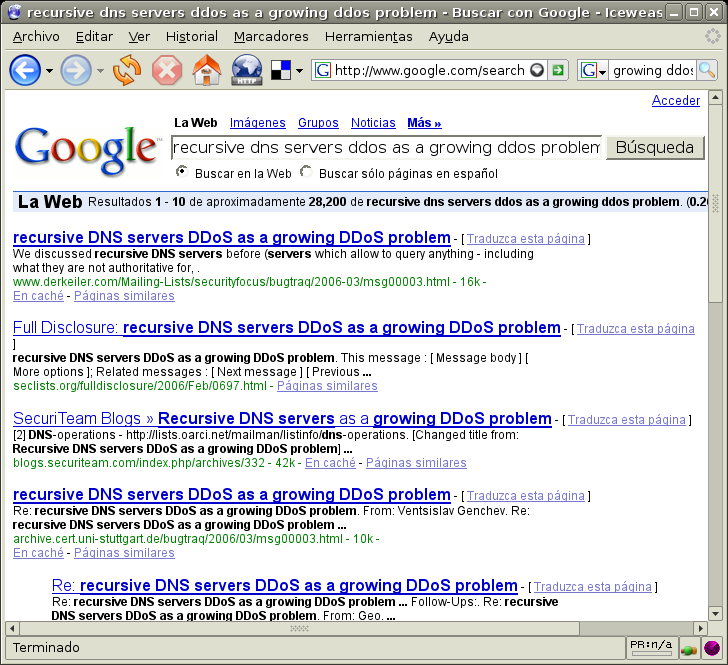
\includegraphics[width=0.9\textwidth]{images/query-google.png}
  \end{center}
}

\section{La Web semántica}
\frame
{
  \frametitle{La Web semántica}

  \begin{Large}
    La Web semántica es una \textbf{extensión} sobre la Web actual donde el 
    contentido Web debe ser expresado de forma que sea entendido, interpretado 
    y usado por máquinas.
  \end{Large}
  
  \vspace{1cm}

  \begin{Large}
    Proviene de la visión de Tim Berners-Lee (Director del W3C) de la Web como un
    medio \textbf{universal} para el intercambio de \textbf{datos}, \textbf{información} 
    y \textbf{conocimiento}.
  \end{Large}

  \vspace{1cm}

  \begin{Large}
    La siguiente versión de la Web, la \textbf{Web 3.0}
  \end{Large}
}
\frame
{
  \frametitle{RSS, un caso de uso muy conocido}

  \begin{center}
    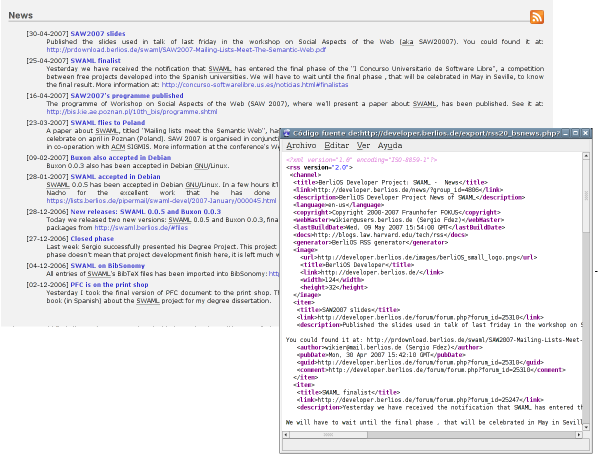
\includegraphics[width=0.95\textwidth]{images/rss.png}
  \end{center}
}
\frame
{
  \frametitle{La pila de la Web semántica}

  \begin{center}
    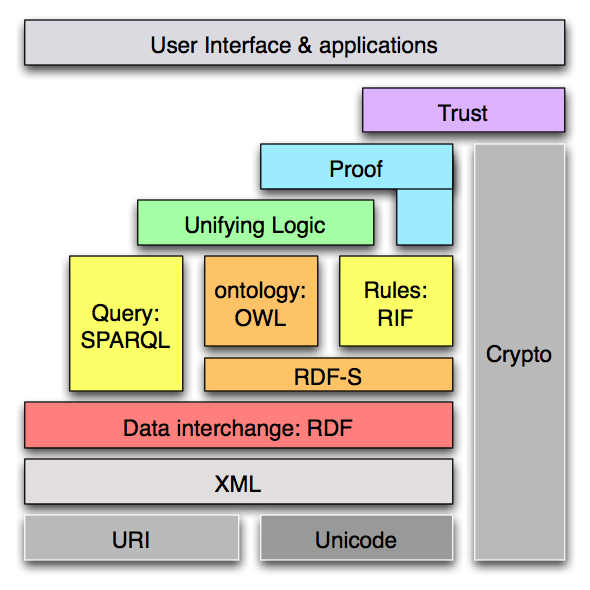
\includegraphics[width=0.8\textwidth]{images/semantic-web-stack.png}
  \end{center}

}
\frame
{
  \frametitle{RDF}

  \begin{Large}
     \textbf{R}esource \textbf{D}escription \textbf{F}ramework es una familia de
     tecnologías (RDF, SPARQL, etc...) de W3C para modelar conocimiento. 
  \end{Large}

  \vspace{0.7cm}

  \begin{Large}
     RDF se basa en un modelo de tripletas:
     \begin{center}
       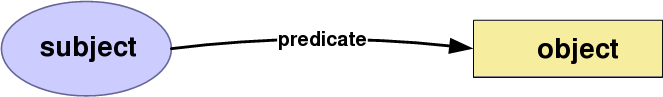
\includegraphics[width=0.8\textwidth]{images/triple.png}
     \end{center}
     El \textbf{sujeto} es un recurso, identificado por un URI 
     (\textit{Uniform Resource Identifier}), que se relaciona mediante un 
     \textbf{predicado} con un \textbf{objeto}, que puede ser a su vez otro 
     recurso o un literal.
  \end{Large}
}
\frame
{
  \frametitle{SIOC}

  \begin{Large}
    \textbf{S}emantically-\textbf{I}nterlinked \textbf{O}nline \textbf{C}ommunities 
    es una ontologia que provee un vocabulario para interconectar diferente sitios
    de discusión, como blogs, wikis, foros y/o listas de correo.
  \end{Large}

  \begin{center}
    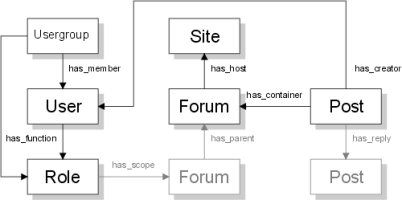
\includegraphics[width=0.8\textwidth]{images/sioc-terms.png}
  \end{center}

}

\section{Herramientas de software}
\frame
{
  \frametitle{Herramientas de software}

  Principalmente hemos desarrollado dos herramientas de software como parte
  de este proyecto:
  \vspace{0.5cm}
  \begin{itemize}
    \item<2->	\begin{Large}\textbf{SWAML} es un aplicación no interactiva
		en linea de comandos cuyo principal propósito es \textit{traducir}
		mailboxes en instancias de \texttt{sioc:Forum} en RDF.\end{Large}
    \vspace{1cm}
    \item<3->	\begin{Large}\textbf{Buxon} es un navegador gráfico para
		visualizar instancias de \texttt{sioc:Forum}.\end{Large}
  \end{itemize}
}
\frame
{
  \frametitle{Herramientas de software}

  \begin{center}
    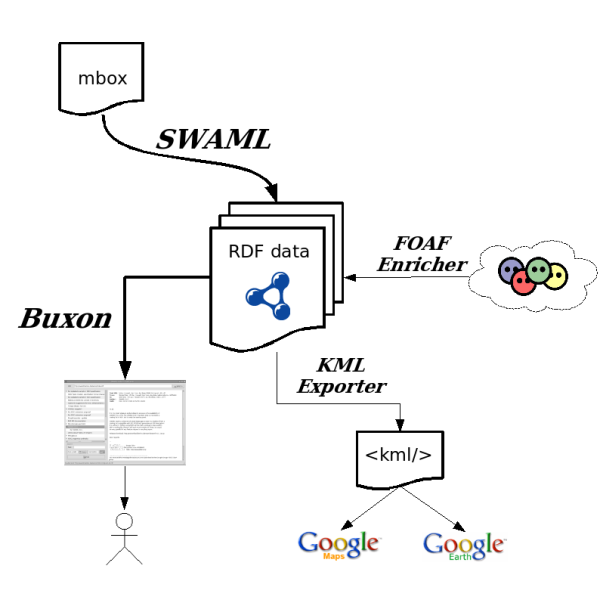
\includegraphics[width=0.85\textwidth]{images/swaml-tools.png}
  \end{center}
}
\frame
{
  \frametitle{SWAML}

  \begin{columns}
   \begin{column}{0.5\textwidth}
	\begin{center}
	  \only<1>{
\includegraphics[width=0.95\textwidth]{images/swaml-0.png}}
	  \only<2>{
\includegraphics[width=0.95\textwidth]{images/swaml-1.png}}
	  \only<3>{
\includegraphics[width=0.95\textwidth]{images/swaml-2.png}}
	  \only<4>{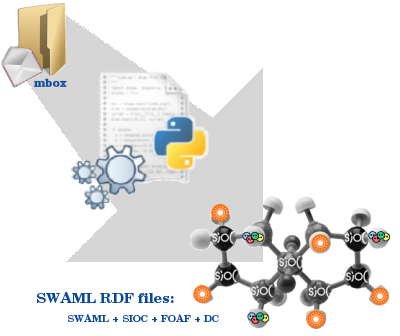
\includegraphics[width=0.95\textwidth]{images/swaml-3.png}}
	\end{center}
   \end{column}
   \begin{column}{0.5\textwidth}
	\begin{Large}proceso batch:\end{Large}
	\begin{enumerate}
	 \item<2-> mbox
	 \item<3-> parser
	 \item<4-> serializar a RDF/XML 
	\end{enumerate}
   \end{column}
  \end{columns}
}
\frame
{
  \frametitle{SWAML y KML}

  SWAML también exporta en KML las coordenadas geográficas de los suscriptores
  de una lista de correo.

  \begin{center}
    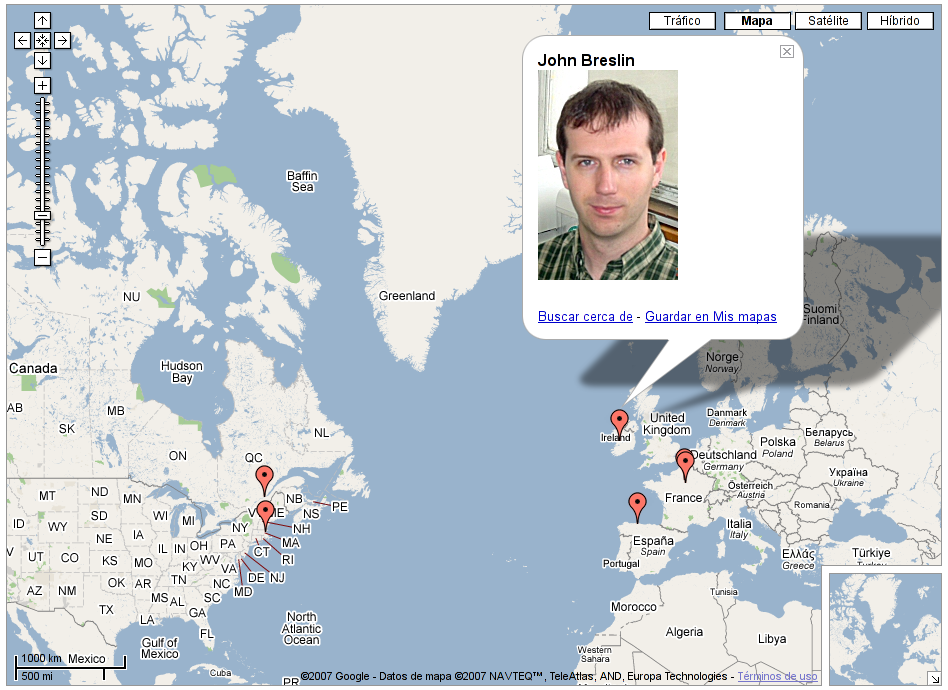
\includegraphics[width=0.7\textwidth]{images/googlemaps.png}\\
    SWAML + SPARQL + FOAF = mash-up!
  \end{center}
}
\frame
{
  \frametitle{Buxon}

  \begin{columns}
   \begin{column}{0.32\textwidth}
	\begin{itemize}
	  \item un lector de \texttt{sioc:Forum}
	  \item recompone los hilos de los mensajes
	  \item quizás la implementaciñon más madura de SIOC
	\end{itemize}
   \end{column}
   \begin{column}{0.68\textwidth}
	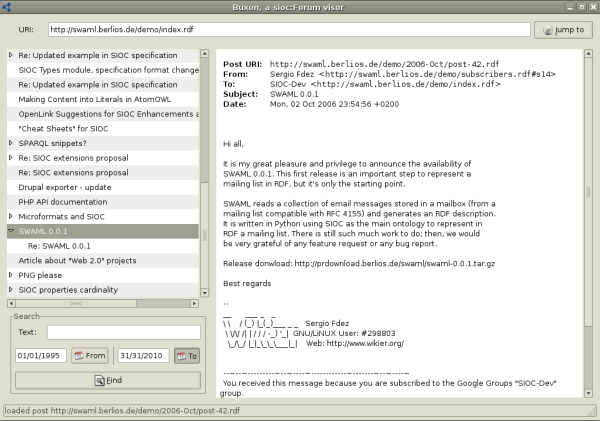
\includegraphics[width=\textwidth]{images/buxon.png}
   \end{column}
  \end{columns}
}

\section{Conclusiones y trabajo futuro}
\frame
{
  \frametitle{Conclusiones técnicas}

  \begin{itemize}
   \item \begin{Large}Conseguir que la inmensa cantidad de conocimiento que almacenan
	 las distintas listas de correo pueda llegar a ser \textbf{útil} de 
         verdad.\end{Large}
   \vspace{1cm}
   \item \begin{Large}Apoyo a la submission de SIOC al W3C.\end{Large}
   \vspace{1cm}
   \item \begin{Large}Presencia internacional (paquetes en Debian GNU/Linux)
	 con una relativa comunidad ya.\end{Large}
  \end{itemize}

}
\frame
{
  \frametitle{Conclusiones personales}

  \begin{itemize}
   \item \begin{Large}Mayor involucración en la comunidad del Software Libre\end{Large}
   \vspace{1cm}
   \item \begin{Large}El haber llegado a esta fase final\end{Large}
   \vspace{1cm}
   \item \begin{Large}Y conseguir un título :-)\end{Large}
  \end{itemize}

}
\frame
{
  \frametitle{Trabajo futuro}

  \begin{itemize}
   \item \begin{Large}Generar RDFa, incluyendo las tripletas en el marcado XHTML.\end{Large}
   \vspace{1cm}
   \item \begin{Large}Acceso a cuentas POP/IMAP para no depender de quien aloja la lista de correo.\end{Large}
   \vspace{1cm}
   \item \begin{Large}Publicar los datos a través un SPARQL endpoint.\end{Large}
  \end{itemize}
}

\frame
{

  \begin{quote}
    \begin{Large}
      La tarea de la universidad no es ofrecer lo que la sociedad demanda, 
      sino lo que la sociedad necesita.
    \end{Large}
    \begin{flushright}E. W. Dijkstra\end{flushright}
  \end{quote}

  \vspace{1cm}

  \begin{Large}
    Y como el Software Libre es algo que ayuda a que una sociedad sea mejor, 
    \textbf{la Universidad debe apostar por el Software Libre} para que estos
    beneficios lleguen a la sociedad.
  \end{Large}

}


\frame
{

  \begin{center}
     \begin{Large}¿preguntas...?\end{Large}
  \end{center}

}

\appendix

\section{Agradecimientos}
\frame
{
  \frametitle{Agradecimientos}

  \begin{Large}
    En primer lugar a todas las personas que han puesto su granito de arena en el 
    proyecto, especialmente a \textbf{Diego Berrueta} y \textbf{Jose E. Labra}, 
    pero también a John Breslin y Uldis Bojars de DERI Galway, y a Nacho Barrientos.
  \end{Large}

  \vspace{1cm}

  \begin{Large}
    Y también a los organizadores, patrocinadores y colaboradores del concurso.
  \end{Large}

}

\section{Más información}
\frame
{
  \begin{center}
    Más información en la página Web del proyecto:\\
    \vspace{1cm}
    \LARGE{\href{http://swaml.berlios.de/}{http://swaml.berlios.de/}}\\
  \end{center}

}

\section{Licencia}
\frame
{
  \begin{center}
    \LARGE{%
	\textbf{SWAML}\\
	\textbf{Semantic Web Archive\\of Mailing Lists}
    }\\
    \vspace{1cm}
    \vspace{1cm}
    \begin{tiny}
	Esta charla se distribuye bajo los términos de la licencia:\\
	\textbf{CreativeCommons}\\
	
\includegraphics[width=3.5cm]{images/creativecommons.png}
    \end{tiny}
  \end{center}
}

\end{document}
